% ----------------------------  START --------------------------- 
\documentclass[../main]{subfiles} % main refers to main.tex
\graphicspath{{\subfix{../Illustrations}}}
\begin{document}
\addto\extrasfrench{\protected\edef:{\unexpanded\expandafter{:}}}
\selectlanguage{french}
% --------------------------------------------------------------- 
% Nombre de \contigs avec au moins n \SNP. L'ordonnée indique le nom de l'espèce considérée (\ref{model_bio}) et l'abscisse le \NbSNP considéré.  L'échelle de couleur indique le nombre de \contigs contenant ce \NbSNP.

\newgeometry{left=1cm, right=1cm, top=3cm, bottom=3cm}
\begin{landscape}
\begin{figure}[p]
    \centering
    \begin{subfigure}[b]{0.55\paperwidth}
        \centering
        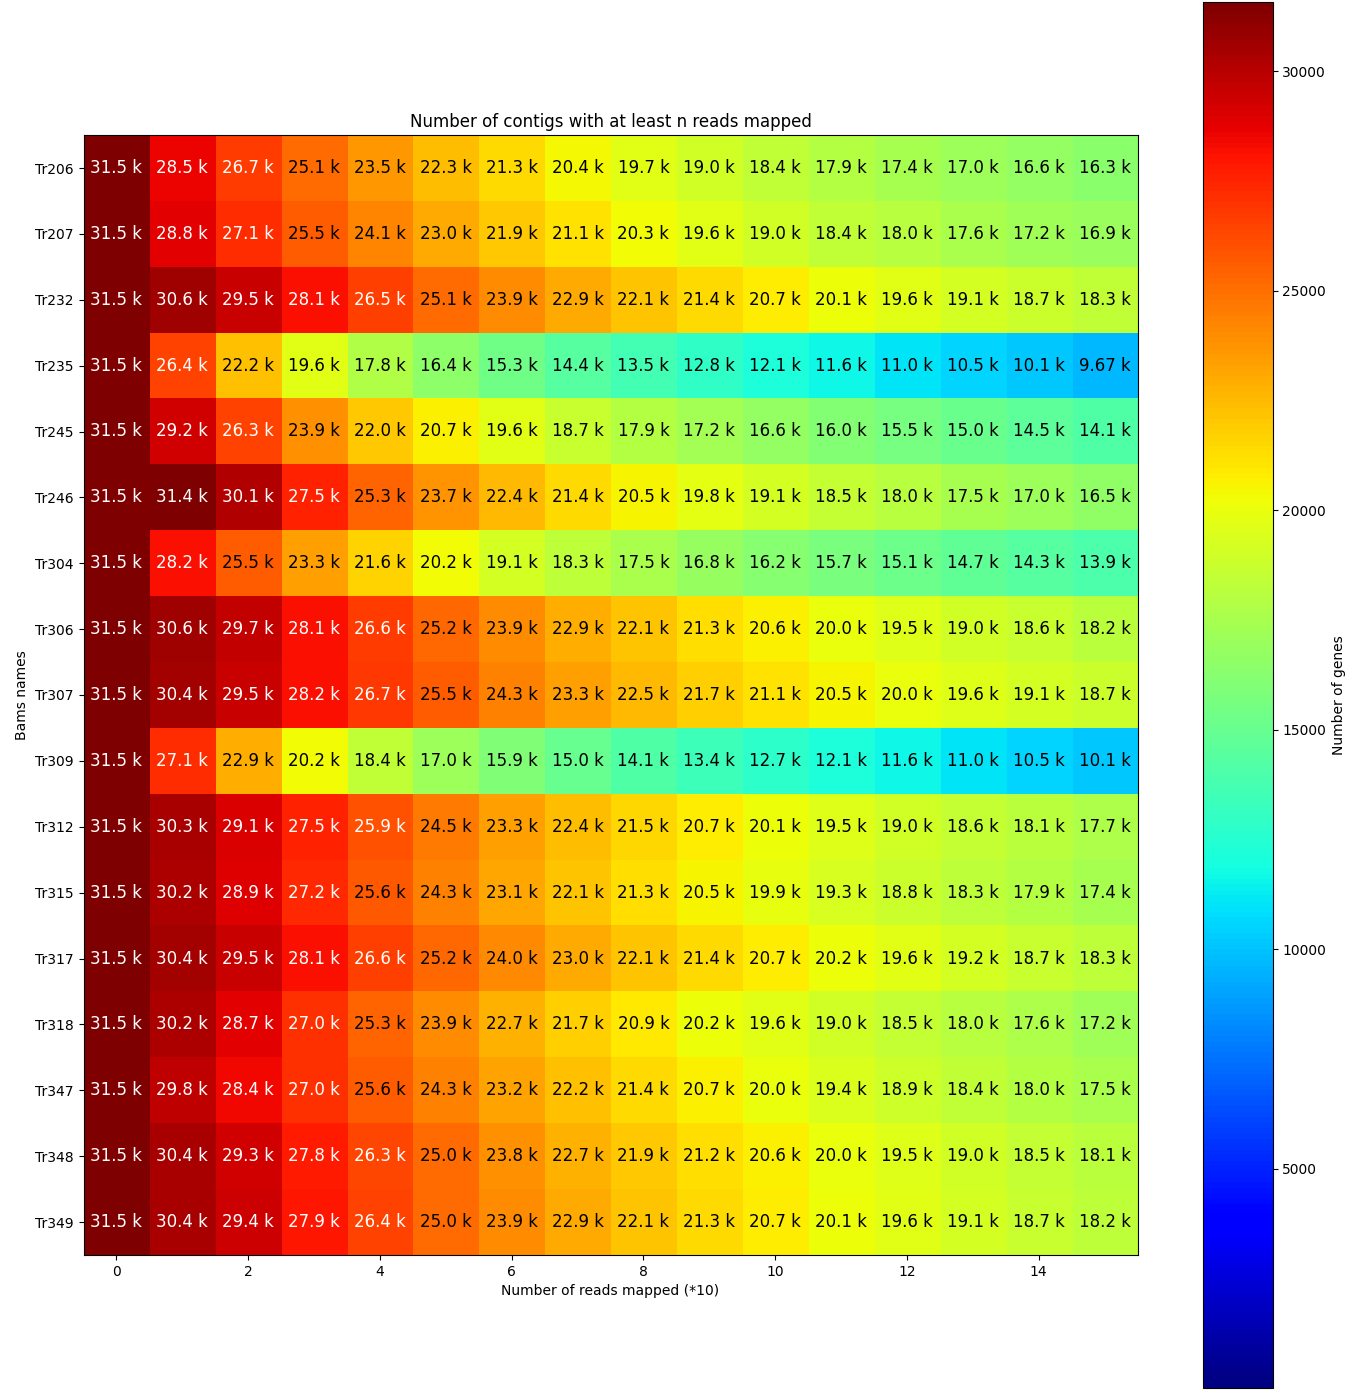
\includegraphics[width=\textwidth]{../Illustrations/Ex_Analysis_Contig_Heatmap_global.png}
        \caption{Résultat de l'analyse des \BamTrEx (\ref{sec:NbReadsParCotigs}).\\
        Commande : \lstinline{Contig Number ./TargetedFiles.json -m 16 -kgqcuwt -j Classic --show_values -1 -y --transparent --legends legends.json --start_at_0}  
        }
        \label{fig:ContigsExClassic}
    \end{subfigure}
    \hfill
    \begin{subfigure}[b]{0.55\paperwidth}
        \centering
        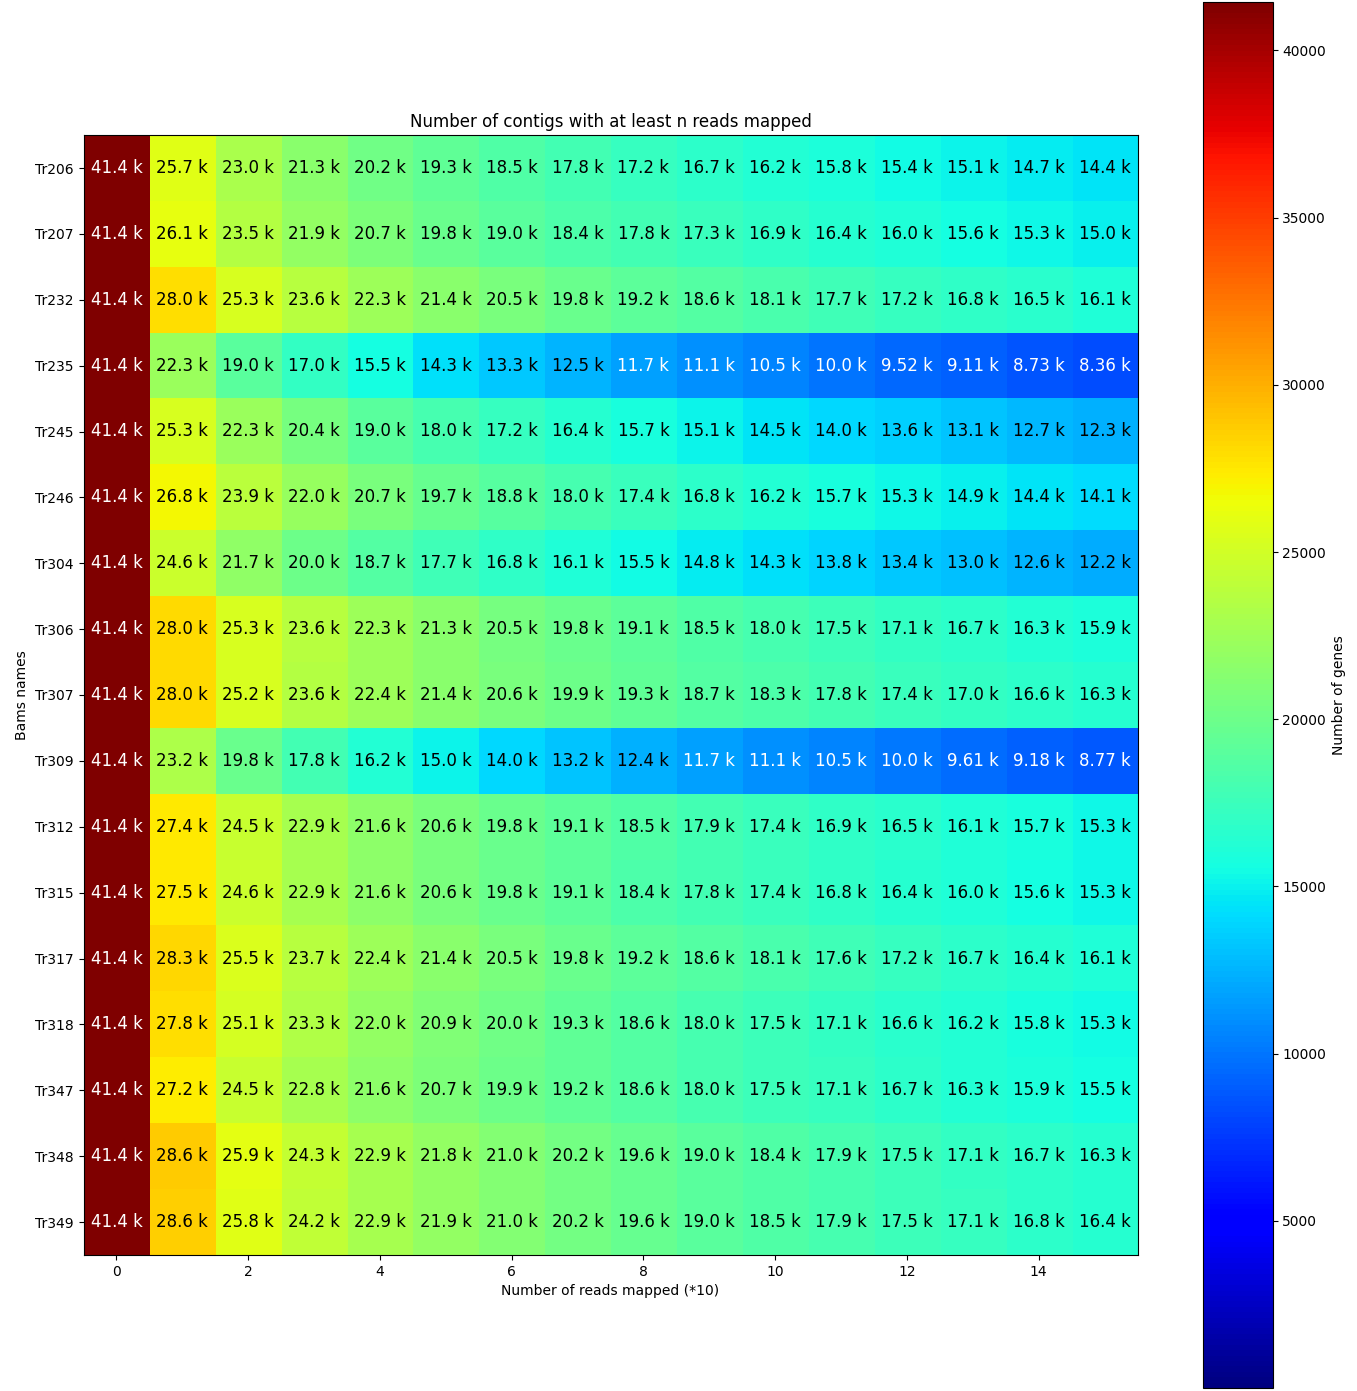
\includegraphics[width=\textwidth]{../Illustrations/Mo_Analysis_Contig_Heatmap_global.png}
        \caption{Résultat de l'analyse des \BamTrMo (\ref{sec:NbReadsParCotigs}).\\
        Commande : \lstinline{Contig Number ./TargetedFiles.json -m 16 -kgqcuwt -j Classic --show_values -1 -y --transparent --legends legends.json --start_at_0}  
        }
        \label{fig:ContigsMoClassic}
    \end{subfigure}
    
      \caption{Résultat de l'analyse des \bam effectuée dans la \ref{sec:NbReadsParCotigs}. Présente le nombre de \contigs avec au moins $n * 10$ \reads dans \BamTrEx et \BamTrMo. L'ordonnée indique le nom de l'individu et l'abscisse le nombre de \reads considéré ($n$). Une incrémentation de $1$ dans l'axe de l'abscisse équivaut à une augmentation de $10$ \reads. L'échelle de couleur indique le nombre de \contigs contenant ce nombre de \reads. \\ Fait avec le logiciel mentionné dans la \ref{sec:SnpHeatmap}. La version utilisée est la 1.2.0.}
    \label{fig:ContigClassicHeatmap}
    
\end{figure}
\end{landscape}
\restoregeometry
% --------------------------------------------------------------- 
\end{document}
% ----------------------------  END --------------------------- 
